\documentclass{article}
\usepackage[T1]{fontenc}
\usepackage{amssymb}
\usepackage{listings}
\usepackage[utf8x]{inputenc}
\usepackage{amsmath,amssymb}
\usepackage{pdfpages}
\usepackage[russian,english]{babel}
\lstset{
    language=Octave,
    frame=single
}
\usepackage[a4paper,top=1cm,bottom=2cm,left=1.5cm,right=1cm,marginparwidth=1.75cm]{geometry}

\makeatletter
\def\@seccntformat#1{
  \expandafter\ifx\csname c@#1\endcsname\c@section\else
  \csname the#1\endcsname\quad
  \fi}
\makeatother

\begin{document}

\selectlanguage{russian}
\title{Лабораторная работа 3, ТВМС}
\author{
	Бочарников Андрей, M3238\\
	Ковешников Глеб, M3238\\
	Шишкин Алексей, M3238
}
\maketitle

\begin{quote}
\selectlanguage{russian}
\section{Формулировка}
	Для случайной величины, распределенной по нормальному закону с параметрами ($a$,$\sigma^2$), выполнить следующие действия:\\\\
	1. Задать параметры распределения $X \thicksim N(a, \sigma^2)$.\\
	2. Построить график $F_x(x)$.\\
	3. Построить выборку генеральной совокупности $X$.\\
	4. По построенной выборке построить график эмпирической функции распределения $F_n(x)$.\\
	5. Построить доверительную полосу надежности.\\
	6. На этом же графике построить $F_n(x)$ и $F_x(x)$.\\
	7. На основе критерия Колмогорова провести проверку гипотез.\\\\
	Аналогично для $X \thicksim U(a, b)$ - равномерно распределенной на $[a, b]$ случайной величины.
\section{Входные данные}
        \begin{itemize}
            \item Выборка генеральной совокупности: $n = 100$
	    \item Доверительная полоса надежности: $\alpha = 0.05$, $u(1 - \alpha) = 1.36$
            \item Проверка критерия Колмогорова: $n = 10^4$ и $10^6$
        \end{itemize}
\section{Программа 1}
	Нормальное распределение.\\ \\
        \begin{minipage}{\linewidth}
            \lstinputlisting{task1.m}
        \end{minipage}
	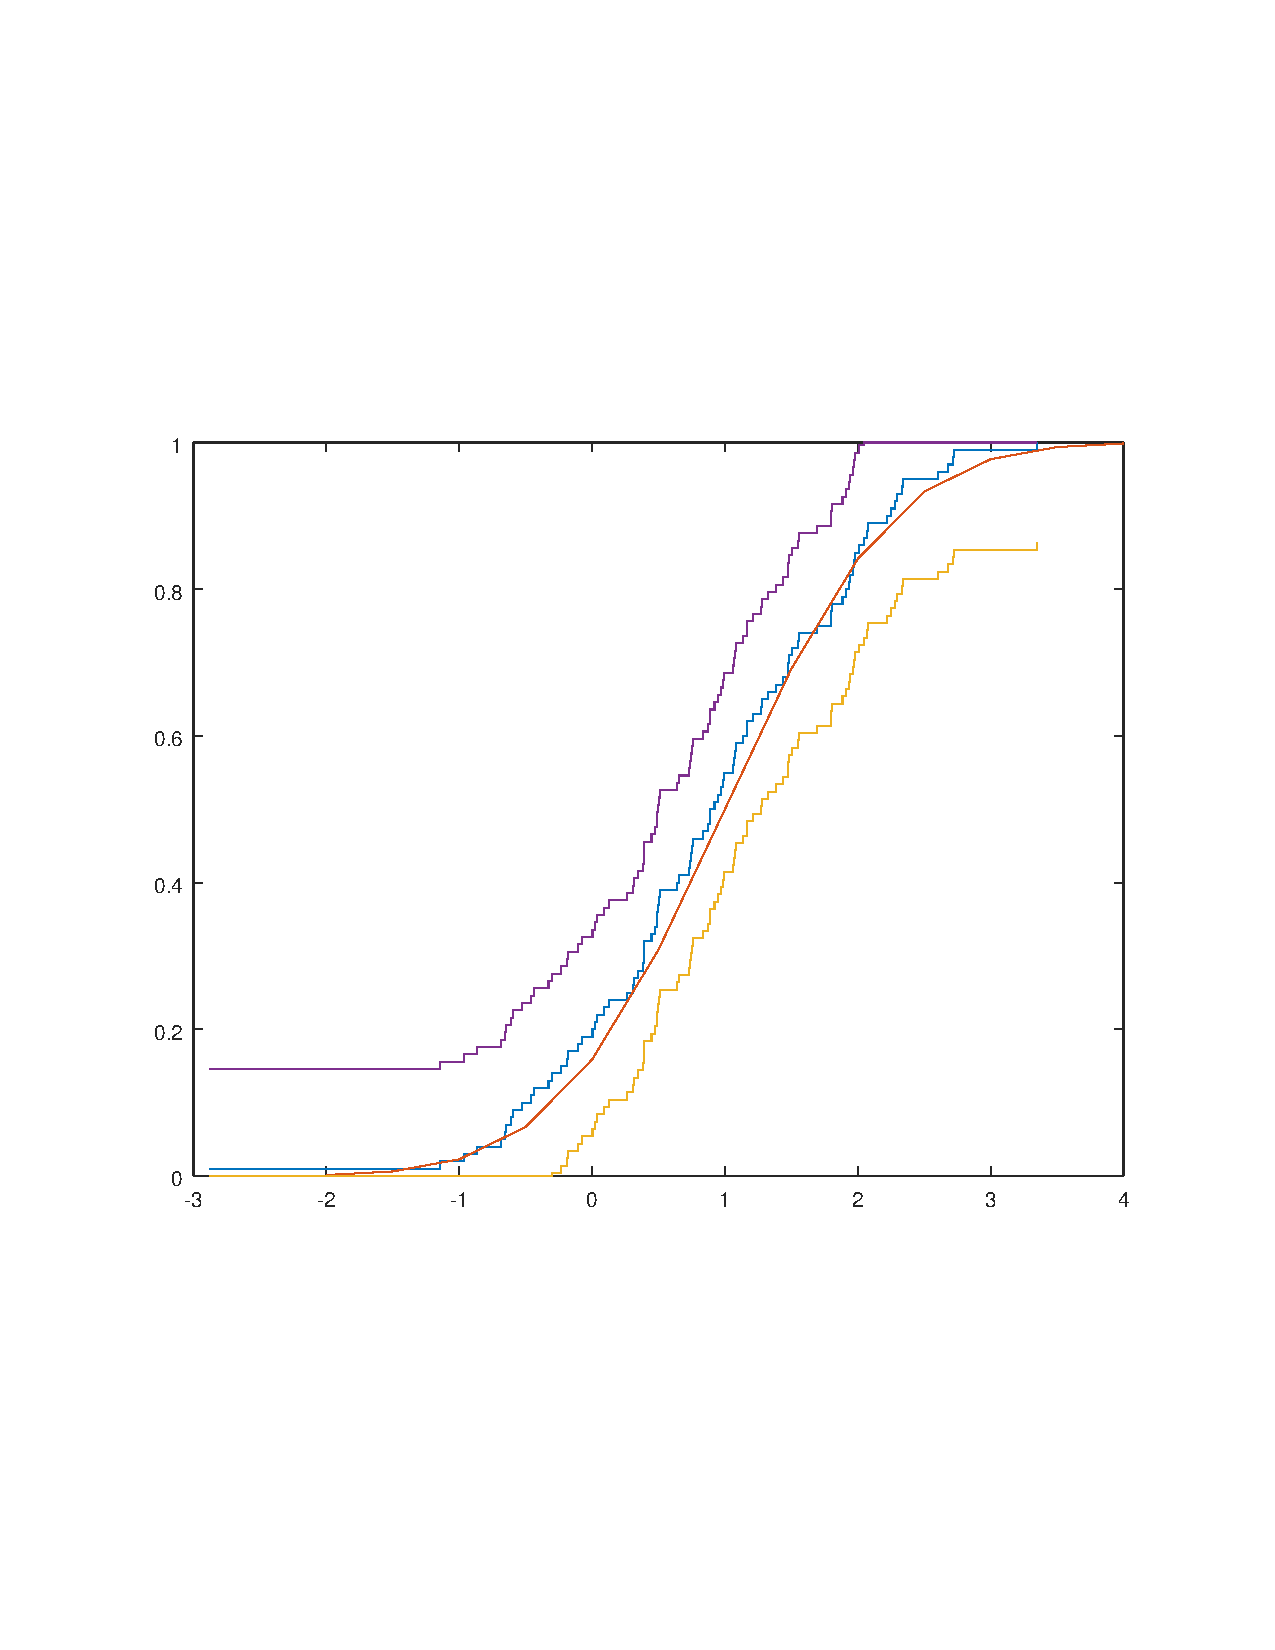
\includepdf[pages=-,pagecommand={},width=\textwidth]{normal_grafic.pdf}
\section{Программа 2}
	Равномерное распределение.\\ \\
        \begin{minipage}{\linewidth}
	    \lstinputlisting{task2.m}
        \end{minipage}
	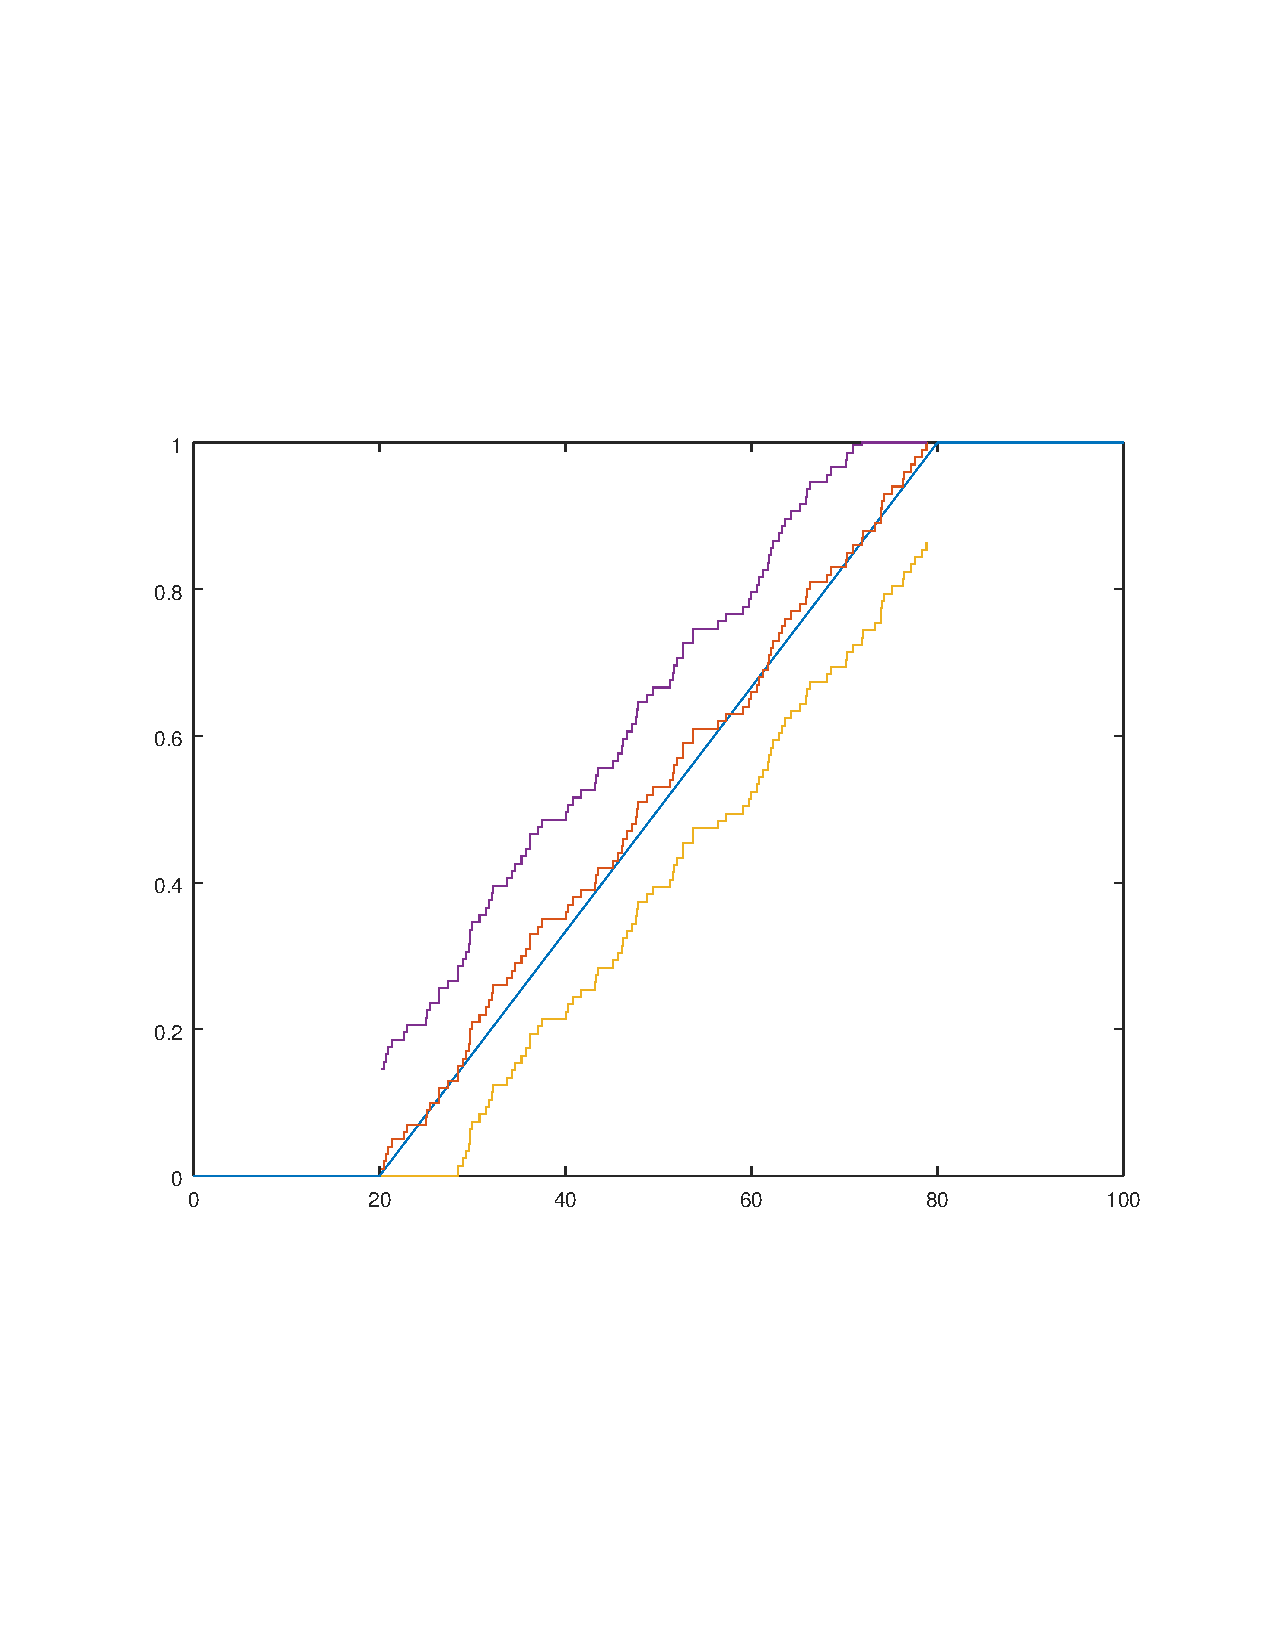
\includepdf[pages=-,pagecommand={},width=\textwidth]{uniform_grafic.pdf}
\section{Проверка гипотез}
        И для нормального, и для равномерного распределения результаты получаются одинаковые:\\
        На основе критерия Колмогорова с параметром $\alpha = 0.05$, вероятность ошибки первого рода асимптотически получается какой и должна быть -- $0.0448$ и $0.45$ при $n=10^4$ и $n=10^6$ соответственно. \\
        На основе критерия Смирнова с параметром $\alpha = 0.01$, вероятность ошибки первого рода при $n=10^4$ и $n=10^6$ получается $0.0148$ и $0.12374$ соответственно, то есть сходится к $0.01$, как и должно быть.
\section{Вывод}
	В обоих распределениях, видно по графикам, что функция распределения лежит в доверительной полосе. Гипотезы также сходятся к нужным величинам.
\end{quote}
\end{document}
